\lecture{10}{13. April 2026}{The De Saint Venant Problem, Pt. I}

\section{The De Saint Venant Problem}

\subsubsection{The Saint-Venant Assumptions}
We consider a straight cylinder whose axis is in the $\Vec{e}_3$-direction and with a cross section in the $\Vec{e}_1 \Vec{e}_2$-plane as shown on \Cref{fig:dsv1}.

\begin{figure} [ht]
  \centering
  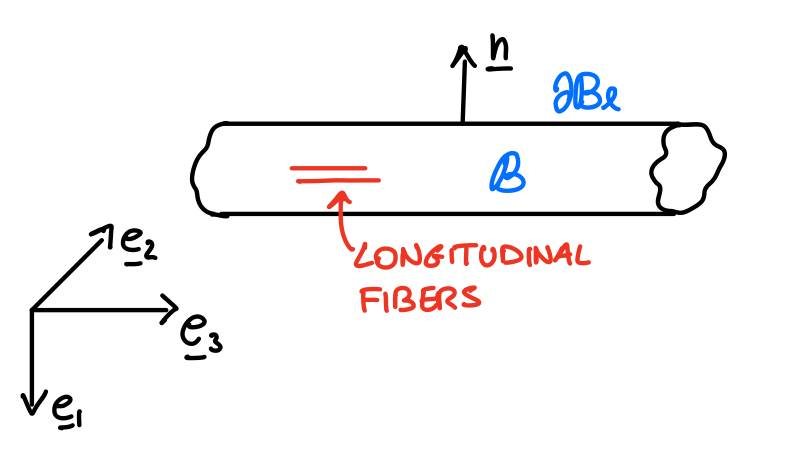
\includegraphics[width=0.5\linewidth]{./figures/dsv1.png}
  \caption{Straight cylinder}
  \label{fig:dsv1}
\end{figure}

The boundary of this cylinder is split into:
\begin{equation*}
  \partial B = \partial B_{l} \cup \partial B_e
\end{equation*}
where, $\partial B_l $ is the lateral surface and $\partial B_e$ is the end/base surface.
The outward normal on the lateral surface satisfies
\begin{equation*}
  \Vec{n} \cdot \Vec{e}_3 = 0
\end{equation*}
because the lateral surface normal has no component in the beam axis direction. 

The assumptions are:
\begin{enumerate}
  \item No loads on the lateral surface
    \begin{equation*}
      \sigma \Vec{n} = 0, \qquad \text{on } \partial B_l
    .\end{equation*}
    So the sides of the beam are traction-free.
  \item Loads only act on the end faces.
    This means external loading is applied only at the bases/cross-sections.
  \item Longitudinal fibers only exchange tangential stresses.
    I.e. if we imagine the cylinder as a bundle of fibres running along $\Vec{e}_3$, then between neighboring fibres, the model only allows tangential interaction, not normal compression between fibers.
\end{enumerate}
Mathematically, for every normal vector $\Vec{n}$ lying in the $\Vec{e}_1 \Vec{e}_2$-plane,
\begin{equation*}
  \Vec{n} \cdot \sigma \Vec{n} = 0, \qquad \forall \Vec{n} : \Vec{n} \cdot \Vec{e}_3 = 0
.\end{equation*}
So if
\begin{equation*}
  \Vec{n} = \begin{pmatrix}
    n_1\\
  n_2\\
  0\\
  \end{pmatrix}
\end{equation*}
then
\begin{equation*}
  \Vec{n} \cdot \sigma \Vec{n} = \sigma_{11} n_1^2 + 2\sigma_{12}n_1n_2 + \sigma_{22}n_2^2
.\end{equation*}
For this to be zero for all choices of $n_1, n_2$, every coefficient must vanish:
\begin{equation*}
  \sigma_{11} = \sigma_{22} = \sigma_{12} = 0
.\end{equation*}
So the stress tensor loses all the purely in-plane stress components. 

\subsubsection{Simplified Cauchy Stress Tensor}
Because of the assumptions mentioned above, the Cauchy stress tensor reduces to:
\begin{equation*}
  \sigma = \begin{bmatrix}
    0 & 0 & \sigma_{31}\\
  0 & 0 & \sigma_{31}\\
  \sigma_{31} & \sigma_{32} & \sigma_{33}\\
  \end{bmatrix}
.\end{equation*}
The remaining stresses are, $\sigma_{31}$ and $\sigma_{32}$, which are shear stresses and $\sigma_{33}$ which is the normal stress in the beam direction. 

So the stress state is much simpler now.
The beam can carry axial normal stress, $\sigma_{33}$ and shear stresses $\sigma_{31}$ and $\sigma_{32}$, but not in-plane stresses like $\sigma_{11}, \sigma_{22}, \sigma_{12}$.

For a plane with normal vector
\begin{equation*}
  \Vec{n} = \begin{pmatrix}
    n_1\\
  n_2\\
  n_3\\
  \end{pmatrix}
\end{equation*}
the traction vector acting on the plane is
\begin{equation*}
  \Vec{T}_n = \sigma \Vec{n}
.\end{equation*}
Using the simplified stress tensor, this can be written as:
\begin{equation*}
  \Vec{T}_n = \begin{pmatrix}
    \sigma_{31}n_3\\
  \sigma_{32}n_3\\
  \sigma_{31} n_1 + \sigma_{32} n_e + \sigma_{33} n_e\\
  \end{pmatrix} = \begin{pmatrix}
    \sigma_{31}n_3\\
  n_{32}n_3\\
  0\\
  \end{pmatrix} + \begin{pmatrix}
    0\\
  0\\
  \sigma_{31}n_1 + \sigma_{32} n_2 + \sigma_{33} n_3\\
  \end{pmatrix}
.\end{equation*}
In the above, the first part is related to shear in the cross section and the second part acts in the longitudinal direction $\Vec{e}_3$. 

An important special case is a cut perpendicular to the cylinder acis,
\begin{equation*}
  \Vec{n} = \Vec{e}_3 = \begin{pmatrix}
    0\\
  0\\
  1\\
  \end{pmatrix}
\end{equation*}
so
\begin{equation*}
  \Vec{T}_{\Vec{e}_3} = \sigma \Vec{e}_3 = \begin{pmatrix}
    \sigma_{31}\\
  \sigma_{32}\\
  \sigma_{33}\\
  \end{pmatrix}
.\end{equation*}
I.e. the traction on a cross section is made up of the shear stress components $\sigma_{31}, \sigma_{32}$ and the axial/normal stress component $\sigma_{33}$.

\subsection{Equilibrium Equations}
Without body forces, the local equilibrium equation is
\begin{equation*}
  \mathrm{div}\, \sigma = \Vec{0}
\end{equation*}
which in index notation is
\begin{equation*}
  \sigma_{ij,j} = 0
.\end{equation*}
Using the simplified stress tensor, this becomes the following three equations:
\begin{align*}
  \sigma_{31,3} &= 0 \\
  \sigma_{32,3} &= 0 \\
  \sigma_{31,1} + \sigma_{32,2} + \sigma_{33,3} &= 0
.\end{align*}
I.e. the shear stresses $\sigma_{31}$ and $\sigma_{32}$ do not vary along the length of the cylinder.
By defining the shear vector on the cross section as:
\begin{equation*}
  \Vec{\tau}_3 = \begin{pmatrix}
    \sigma_{31}\\
  \sigma_{32}\\
  \end{pmatrix}
\end{equation*}
the equations can be rewritten as:
\begin{align*}
  \Vec{\tau}_{3,3} &= \Vec{0} \\
  \mathrm{div}\, \Vec{\tau}_3 &= - \sigma_{33,3}
.\end{align*}

\subsubsection{Boundary Condition on the Lateral Surface}
On the lateral surface,
\begin{equation*}
  \Vec{n} \cdot \Vec{e}_3 = 0
,\end{equation*}
so
\begin{equation*}
  \Vec{n} = \begin{pmatrix}
    n_1\\
  n_2\\
  0\\
  \end{pmatrix}
.\end{equation*}
The traction is then:
\begin{equation*}
  \sigma \Vec{n} = \begin{bmatrix}
    0 & 0 & \sigma_{31}\\
  0 & 0 & \sigma_{32}\\
  \sigma_{31} & \sigma_{32} & \sigma_{33}\\
  \end{bmatrix} \begin{pmatrix}
    n_1\\
  n_2\\
  0\\
  \end{pmatrix} = \begin{pmatrix}
    0\\
  0\\
  \sigma_{31} n_1 + \sigma_{32} n_2\\
  \end{pmatrix}
.\end{equation*}
For the lateral surface to be traction free we have that:
\begin{equation*}
  \sigma \Vec{n} = \Vec{0}
.\end{equation*}
Therefore,
\begin{equation*}
  \sigma_{31}n_1 + \sigma_{32}n_2 = 0
\end{equation*}
now, using $\Vec{\tau}_3$, this becomes
\begin{equation*}
  \Vec{\tau}_3 \cdot \Vec{n} = 0
.\end{equation*}
So the shear stress vector $\Vec{\tau}_3$ must be tangent to the boundary of the cross-section.

\subsubsection{Resultant Force on a Cross-Section}
Now we move form local stresses to global force resultants.

On a cross section $S$, with normal $\Vec{e}_3$, the traction vector is
\begin{equation*}
  \Vec{T}_{\Vec{e}_3} = \begin{pmatrix}
    \sigma_{31}\\
  \sigma_{32}\\
  \sigma_{33}\\
  \end{pmatrix}
.\end{equation*}
The resultant force is the integral of traction over the cross section:
\begin{equation*}
  \Vec{R} = \int_{S} \Vec{T}_{\Vec{e}_3} \, \mathrm{d}S
.\end{equation*}
So
\begin{equation*}
  \Vec{R} = \int_S \begin{pmatrix}
    \sigma_{31}\\
  \sigma_{32}\\
  \sigma_{33}\\
  \end{pmatrix} \, \mathrm{d}S = \begin{pmatrix}
    \int_S \sigma_{31} \, \mathrm{d}S\\
  \int_S \sigma_{32} \, \mathrm{d}S\\
  \int_S \sigma_{33} \, \mathrm{d}S\\
  \end{pmatrix}
.\end{equation*}
We can label this as:
\begin{equation*}
  \Vec{R} = \begin{pmatrix}
    T_1\\
  T_2\\
  N\\
  \end{pmatrix}
,\end{equation*}
where $T_1$ is the shear force in the $e_1$ direction, $T_2$ is the shear force in the $e_2$ direction and $N$ is the axial normal force.


\subsubsection{Resultant Moment on a Cross-Section}
The moment resultant about the barycenter $G$  of the cross-section is
\begin{equation*}
  \Vec{M} = \int_S \left( \Vec{x} - \Vec{x}_G \right) \times \Vec{T}_{\Vec{e}_3} \, \mathrm{d}S
.\end{equation*}
The vector
\begin{equation*}
  \Vec{x} - \Vec{x}_G
\end{equation*}
is the position vector from the centroid of the cross-section to the point where the stress acts.

In the cross-section,
\begin{equation*}
  \Vec{x}- \Vec{x}_G = \begin{pmatrix}
    x_1\\
  x_2\\
  0\\
  \end{pmatrix}
\end{equation*}
the traction is
\begin{equation*}
  \Vec{T}_{\Vec{e}_3} = \begin{pmatrix}
    \sigma_{31}\\
  \sigma_{32}\\
  \sigma_{33}\\
  \end{pmatrix}
.\end{equation*}
So the cross-product is
\begin{equation*}
  \left( \Vec{x} - \Vec{x}_G  \right) \times \Vec{T}_{\Vec{e}_3} = \begin{pmatrix}
    x_2 \sigma_{33}\\
  - x_1 \sigma_{33}\\
  x_1 \sigma_{32} - x_2 \sigma_{31}\\
  \end{pmatrix}
.\end{equation*}
We can also write this as:
\begin{equation*}
    \left( \Vec{x} - \Vec{x}_G  \right) \times \Vec{T}_{\Vec{e}_3} = \begin{pmatrix}
      \sigma_{33}y\\
    - \sigma_{33} x\\
    x_1 \sigma_{32} - x_2 \sigma_{31}\\
    \end{pmatrix}
.\end{equation*}
The interpretation is:
\begin{equation*}
  M_1 = \int_S x_2 \sigma_{33} \, \mathrm{d}S
\end{equation*}
is a bending moment about $e_1$,
\begin{equation*}
  M_2 = \int_S - x_1 \sigma_{33} \, \mathrm{d}S
\end{equation*}
is a bending moment about $e_2$, and 
\begin{equation*}
  M_3 = \int_S \left( x_1 \sigma_{32} - x_2 \sigma_{31} \right) \, \mathrm{d}S
\end{equation*}
is the torsional moment about $e_3$.

\subsection{The Saint-Venant Principle}
The Saint-Venant principle states that ``statically equivalent force systems acting on the base surfaces of a straight cylinder give rise to the same stress/strain states, except for small regions near the base surfaces.''

This means, that if two different load distributions have the same resultant force and moment, than far enough away from the loaded ends, the body ``does not care'' about the exact details of how the load was applied.


